\documentclass[a4paper, 11pt, titlepage, twoside, openany]{book}
\usepackage{plain}
\usepackage{setspace}
% Layout
\usepackage[
  paperheight=29.7cm,
  paperwidth=21cm,
  outer=1.5cm,
  inner=2.5cm,
  top=2cm,
  bottom=2cm
]{geometry}
% Chapter
\usepackage{titlesec}
\singlespacing
\setcounter{secnumdepth}{3}
\setcounter{tocdepth}{3}
% Letter
\usepackage[utf8]{inputenc}
% Language
\usepackage[italian]{babel}
% PDF/A
\usepackage[a-1b]{pdfx}
% Image
\usepackage{graphicx}
\usepackage{wrapfig}
\usepackage{stackengine}
\usepackage{etoolbox}
\usepackage{subfig}
\BeforeBeginEnvironment{wrapfigure}{\setlength{\intextsep}{0pt}}
% Hyperlink
\usepackage{xurl}
\usepackage[pdfa]{hyperref}
\hypersetup{breaklinks=true}
% List
\usepackage{enumitem}

% Table multi row
\usepackage{multirow}

% Algorithm
\usepackage{algorithm}
\usepackage{algpseudocode}

% Padding
\usepackage{changepage}
\usepackage{varwidth}

\hypersetup{
  breaklinks=true,
  colorlinks=true, % Colora i link invece di usare riquadri colorati
  linkcolor=black, % Colore dei link interni (indice, sezioni)
  citecolor=black, % Colore delle citazioni
  filecolor=black, % Colore dei link ai file locali
  urlcolor=black % Colore degli URL
}

% START: DELETE ME
\usepackage{lipsum}
% END: DELETE ME

% Document
\begin{document}
  % Cover
  \pagenumbering{gobble}
  \pagestyle{plain}

\thispagestyle{empty}

\begin{center}
  \begin{figure}[h!]
    \centering
    
\includegraphics[width=.6\textwidth]{images/logo/unitn.eps}
  \end{figure}

  \vspace{2 cm}

  \LARGE{Dipartimento di Ingegneria e Scienza dell’Informazione\\}

  \vspace{1 cm}
  \Large{Corso di Laurea in\\
    Informatica
  }

  \vspace{2 cm}
  \Large\textsc{Elaborato finale\\}
  \vspace{1 cm}
  \Huge\textsc{Ottimizzazione della libreria Cooperis tramite calcolo parallelo\\}
  \Large{\it{Implementazione e valutazione delle prestazioni dei vari approcci alla parallellizzazione\\}}


  \vspace{2 cm}
  \begin{tabular*}{\textwidth}{ c @{\extracolsep{\fill}} c }
  \Large{Supervisore} & \Large{Laureando}\\
  \Large{Michele Segata}& \Large{Miazzo Luigi}\\
  \ & \Large{226638}\\
  \end{tabular*}

  \vspace{2 cm}

  \Large{Anno Accademico 2023/2024}

\end{center}


  \clearpage

  % Acknowledgements
  %\thispagestyle{empty}
%
\clearpage
\vspace*{\stretch{2}}
\begin{center}
  \begin{flushright}
    \begin{minipage}{.5\textwidth}
      \textit{Alla mia famiglia e ai miei amici per il sostegno, i consigli e i sorrisi
      che mi hanno accompagnato in questo indimenticabile percorso.}
    \end{minipage}
  \end{flushright}
\end{center}
\vspace{\stretch{3}}
\clearpage
  \clearpage
  \pagestyle{plain}

  % Table of Contents
  \frontmatter
  \pagenumbering{Roman}
  \tableofcontents
  \clearpage
  \begingroup
  \pagestyle{empty}
  \cleardoublepage
  \endgroup

  % Start page numbering
  \mainmatter

  % Group to define space between chapters
  \begingroup
  % Override format of title chapter
  \titleformat{\chapter} {\normalfont\Huge\bfseries}{\thechapter}{1em}{} \titlespacing*{\chapter}{0pt}{0.59in}{0.02in}
  \titlespacing*{\section}{0pt}{0.20in}{0.02in} \titlespacing*{\subsection}{0pt}{0.10in}{0.02in}
  \titlespacing*{\subsubsection}{0pt}{0.05in}{0.02in}

  % Abstract
  \chapter*{Abstract}
\label{cha:abtract}
\addcontentsline{toc}{chapter}{Abstract}

Le Reconfigurable Intelligent Surfaces (RISs) sono una tecnologia emergente che
promette di rivoluzionare le comunicazioni wireless del futuro, permettendo di modificare
in tempo reale le caratteristiche del canale di comunicazione tra un trasmettitore
e un ricevitore quando non è possibile instaurare una connessione line-of-sight.
Tuttavia, lo studio e la valutazione della fattibilità e delle prestazioni di questa
tecnologia, come per molte altre, richiede l'utilizzo di strumenti di simulazione
sofisticati e sviluppati ad hoc. I framework di simulazione sono essenziali per
lo studio di tecnologie ancora in uno stato embrionale come le RIS, poiché permettono
di testare e confrontare diverse configurazioni e algoritmi in un ambiente controllato
e riproducibile, evitando costosi test sperimentali, in particolar modo per prodotti
non ancora disponibili sul mercato. Talvolta però, la complessità dei modelli simulativi
e la mole di dati da processare richiedono un'elevata potenza di calcolo e risorse
hardware, che possono risultare insufficienti per ottenere risultati in tempi
ragionevoli. In questo contesto, il calcolo parallelo offre la possibilità di
sfruttare al meglio le risorse a disposizione, riducendo i tempi di esecuzione e
migliorando le prestazioni, tuttavia complicando in alcuni casi la portabilità e
la manutenibilità del codice. Questo elaborato si propone di analizzare tre diversi
framework di programmazione parallela confrontando le principali caratteristiche
che li contraddistinguono, nell'ottica di valutarne l'efficacia, la versatilità,
e ove applicabile la difficoltà d'integrazione. I framework presi in considerazione
sono: parallelizzazione su CPU tramite la libreria \textit{libpthread} e su GPU tramite
le librerie \textit{CUDA} e \textit{OpenCL}. Per questo scopo, è stata eseguita l'integrazione
di ciascuno di questi paradigmi nella libreria \textit{CoopeRIS}, framework di simulazione
per le RISs, al fine di valutarne l'impatto sulle prestazioni delle simulazioni.
I risultati ottenuti da questo studio dimostrano pienamente l'efficacia del calcolo
parallelo, in particolare su GPU, nel ridurre i tempi di esecuzione delle citate
simulazioni, essenzialmente indicando un miglioramento pressoché lineare nella
velocità di esecuzione al crescere del numero di thread utilizzati in
riferimento all'implementazione su CPU, e un incremento di quasi due ordini di grandezza
tramite le implementazioni su GPU.

  % Chapters
  \chapter{Introduzione}
\label{ch:introduzione}

In questo capitolo introduttivo si intende descrivere il contesto e le
motivazioni che hanno portato allo sviluppo di questo elaborato. Si presenta una
panoramica generale del campo di studio in cui l'argomento si colloca, ma non
solo: benché il lavoro svolto si è concentrato su un'implementazione reale, si
vogliono presentare anche l'importanza e i benefici che tali implementazioni e
tecnologie possono portare ad altri algoritmi e applicazioni, ponendo particolare
attenzione ai vantaggi, svantaggi ed eventuali problematiche che sono state
riscontrate durante lo sviluppo. Infine, si presentano gli obiettivi
sperimentali che si intendono raggiungere e la soluzione proposta al fine di
soddisfarli.

\section{Contesto e motivazioni}
\label{sec:contesto}

Gli strumenti di simulazione sono dei meccanismi essenziali nella ricerca tecnologica
e scientifica in quanto il loro utilizzo permette di testare preventivamente le prestazioni
e il comportamento di sistemi estremamente complessi senza dover ricorrere a costose
e rischiose sperimentazioni reali. Anche se il loro utilizzo è molto diffuso, la
loro implementazione non è sempre banale e richiedono un'attenta progettazione e
sviluppo. Per di più, la complessità dei sistemi in esame può portare a realizzare
soluzioni non ottimali e poco efficienti, che, anche se funzionanti e matematicamente
corrette, possono richiedere tempi di esecuzione proibitivi. Questo porta a dover
ricorrere a soluzioni hardware più potenti e costose che riducono il costo-beneficio
dell'intero processo di simulazione. Qui trova spazio l'importanza della
revisione, dell'ottimizzazione e dell'efficientamento del codice, che permettono
di ridurre i tempi di esecuzione e della potenza di calcolo richiesta, permettendo
a una gamma molto più ampia di utenti di poter usufruire di tali strumenti.

\subsection{Reconfigurable Intelligent Surfaces (RISs) e Framework di
simulazione}
\label{subsec:risframework}

\begin{wrapfigure}
  {r}{.40\textwidth}
  \centering
  \def\stackalignment{l}{ 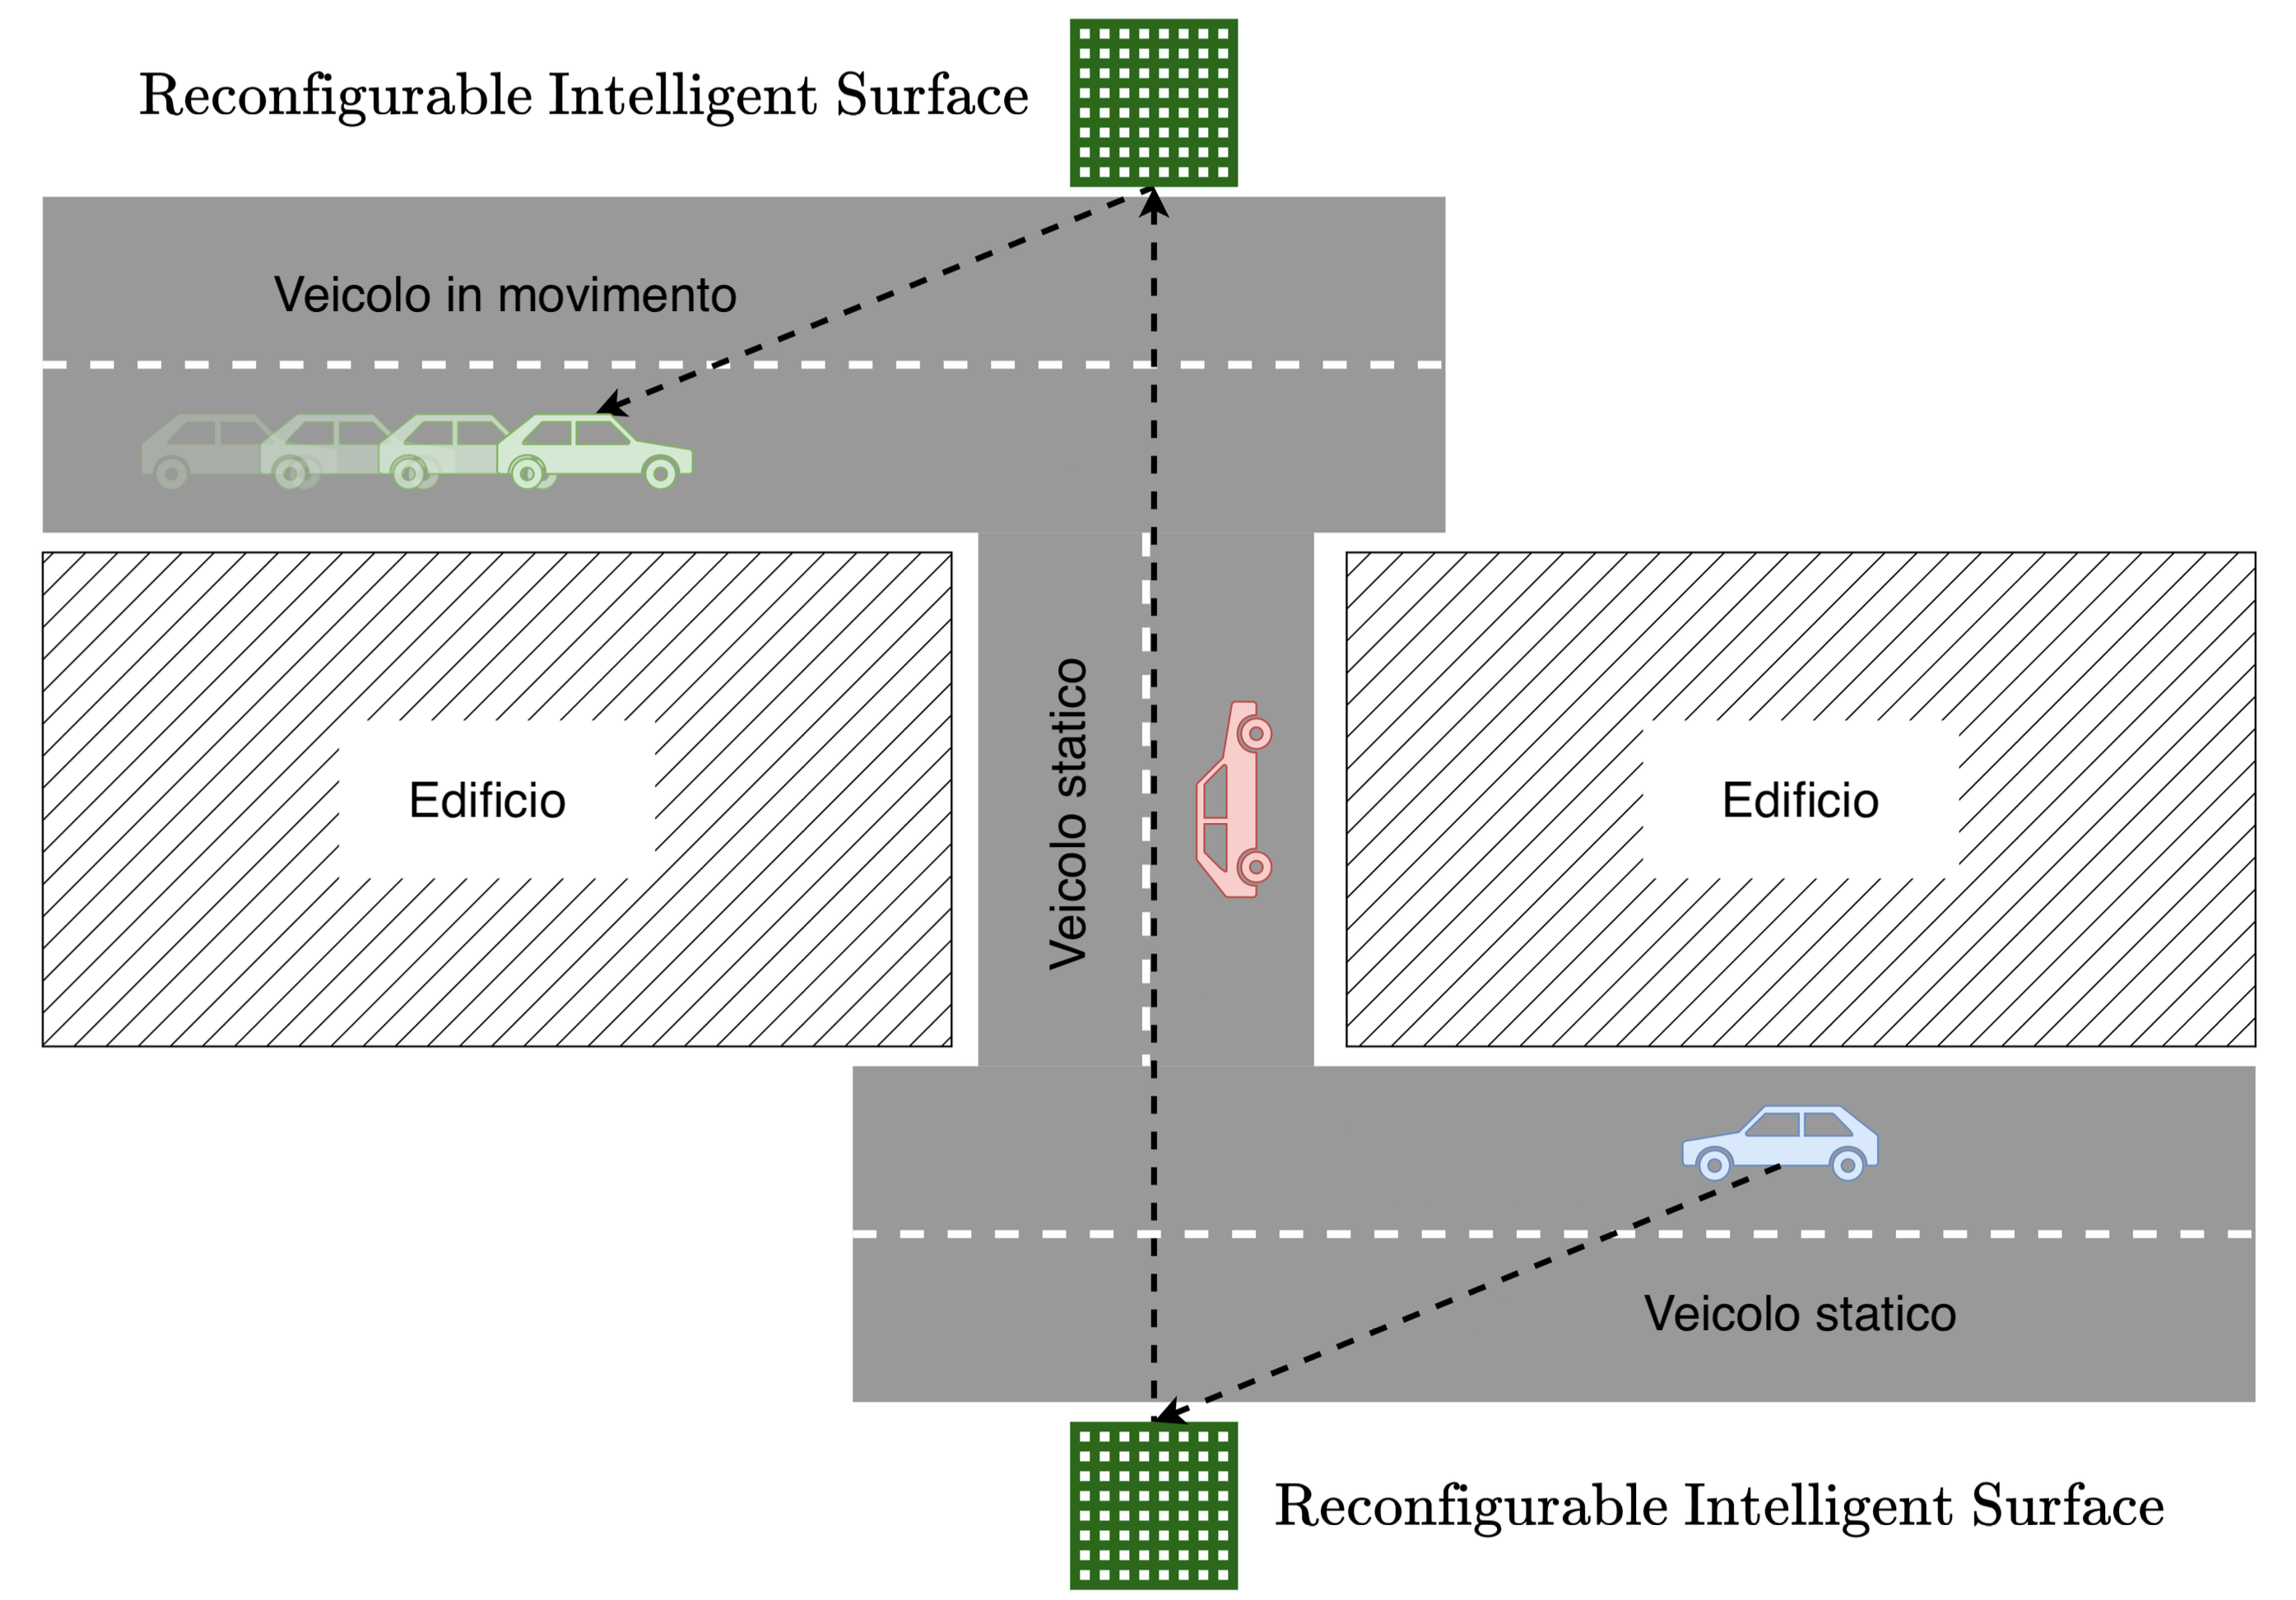
\includegraphics[width=\linewidth]{images/examples/ris-intersection.png} }
  \caption{Scenario di esempio di comunicazione tra veicoli tramite RISs\cite{cooperis}}
  \label{fig:example-ris-scenario}
  \vspace{1em}
\end{wrapfigure}

Le Reconfigurable Intelligent Surfaces (RISs) sono superfici planari programmabili
che permettono di manipolare dinamicamente le loro proprietà di riflessione in modo
da modificare la direzione in cui vengono riflesse le onde elettromagnetiche che
ci interagiscono, di fatto creando il fenomeno del \textit{beamforming}. Possono
essere sia attive, ossia amplificano il segnale riflesso, che passive, le quali si
limitano a riflettere il segnale, e sono essenzialmente costituite da una
griglia di elementi radianti indipendenti, ciascuno dei quali è singolarmente ed
elettronicamente controllabile. Le RISs riscontrano molto interesse nel campo
delle comunicazioni wireless, principalmente nelle reti che sfruttano uno spettro
di frequenze molto elevato, come nelle comunicazioni che utilizzano le onde
millimetriche dove la propagazione e la penetrazione del segnale attraverso gli
ostacoli e le ostruzioni presenti nell'ambiente circostante sono molto scarse, soprattutto
in situazioni in cui non sempre è presente una diretta visibilità (LoS, Line of Sight)
tra trasmettitore e ricevitore, ad esempio in ambienti urbani o indoor. Aumenta
notevolmente la loro utilità quando si considera la loro capacità di
riconfigurazione in tempo reale, permettendo di creare canali di comunicazione dinamici
e più efficienti nei casi in cui ricevitore e trasmettitore siano in movimento,
diminuendo il rumore generato dalla naturale diffusione del segnale e
potenzialmente migliorando la comunicazione tra dispositivi terzi. Questo elaborato
è incentrato sull'ottimizzazione di una libreria sullo studio delle RISs nell'ambito
delle comunicazioni tra veicoli a guida autonoma: in particolare la libreria
\textit{CoopeRIS}\cite{cooperis} permette di simulare il comportamento di queste
superfici nell'ambito delle comunicazioni tra veicoli a guida autonoma. Di seguito
viene citato e descritto brevemente lo stack dei framework di simulazione:
\begin{itemize}
  \item \textit{SUMO} (Simulation of Urban MObility), simulatore di traffico e mobilità
    urbana\cite{sumo};

  \item \textit{OMNeT++} (Objective Modular Network Testbed), simulatore discreto
    ad eventi utilizzato maggiormente nella simulazione di reti\cite{omnetpp};

  \item \textit{Veins} (Vehicles in Network Simulation), simulatore di reti veicolari\cite{veins};

  \item \textit{PLEXE} (PLatooning EXtensions for Veins), estensione di Veins per
    la simulazione del platooning di veicoli\cite{plexe}.
\end{itemize}

\section{Contributo della Tesi}
\label{sec:contributo}

Questo elaborato si pone come obiettivo quello di migliorare la libreria in
oggetto, implementando soluzioni di ottimizzazione ed efficientamento del codice
tramite calcolo parallelo, sia mediante procedure multi-threading che attraverso
l'utilizzo di GPU, con lo scopo finale di ridurre i tempi di esecuzione delle simulazioni.
Inoltre, assieme a queste migliorie, si propone una valutazione sia qualitativa
che quantitativa delle varie tecnologie utilizzate nei casi di studio previsti
dal paper in riferimento\cite{cooperis}, in modo da poter fornire una panoramica
completa delle migliorie ottenute, dei vantaggi e svantaggi di ciascuna tecnologia
e delle problematiche riscontrate durante lo sviluppo. La soluzione proposta
prevede di effettuare un'analisi preventiva del codice sorgente della libreria
in oggetto per identificare le eventuali criticità e i punti in cui una
possibile implementazione di calcolo parallelo potrebbe portare ai miglioramenti
più significativi. In seguito, si procederà con l'implementazione di tre
soluzioni diverse, consultabili alla tabella \ref{tab:soluzioni}, per permettere
la maggior compatibilità con l'hardware a disposizione degli utenti. Per garantire
la correttezza di tutte le implementazioni, il codice sarà testato tramite una
serie di unit test per verificarne la correttezza, e sarà infine inserito all'interno
della libreria utilizzando guardie di precompilazione per permettere la scelta della
tecnologia desiderata.

\vspace{1em}

\begin{table}[ht]
  \begin{center}
    \begin{tabular}{ |c|c|l|l| }
      \hline
      \textbf{Piattaforma} & \textbf{Libreria}   & \textbf{Vantaggi}               & \textbf{Svantaggi}              \\
      \hline
      CPU                  & libpthread          & Facilità di implementazione     & Scalabilità limitata            \\
      \hline
      \multirow{2}{*}{GPU} & CUDA\cite{cuda}     & Elevata potenza di calcolo      & Necessità di hardware specifico \\
      \cline{2-4}          & OpenCL\cite{opencl} & Maggiore compatibilità hardware & Complessità di implementazione  \\
      \hline
    \end{tabular}
    \caption{Soluzioni proposte}
    \label{tab:soluzioni}
  \end{center}
\end{table}
  \chapter{Fondamenti Teorici}
\label{ch:fondamenti}

In questo capitolo verranno trattati alcuni fondamenti teorici necessari per la
comprensione dell'elaborato. Si procederà con un'analisi sullo stato dell'arte della
libreria in oggetto e una breve introduzione al funzionamento delle Reconfigurable
Intelligent Surfaces, per poi passare ad una panoramica generale sulle tecniche
di parallel computing, con particolare attenzione alle differenze tra CPU e GPU e
tra i framework \textit{CUDA} e \textit{OpenCL}. Infine, si presenteranno i presupposti
limiti teorici e risultati attesi.

% do not wrap citation
\section[Modello delle Reconfigurable Intelligent Surfaces]{Modello delle
Reconfigurable Intelligent Surfaces\cite{cooperis}}
\label{sec:statodellarte}

\begin{figure}[!htbp]
  \begin{minipage}[t]{0.5\linewidth}
    \centering
    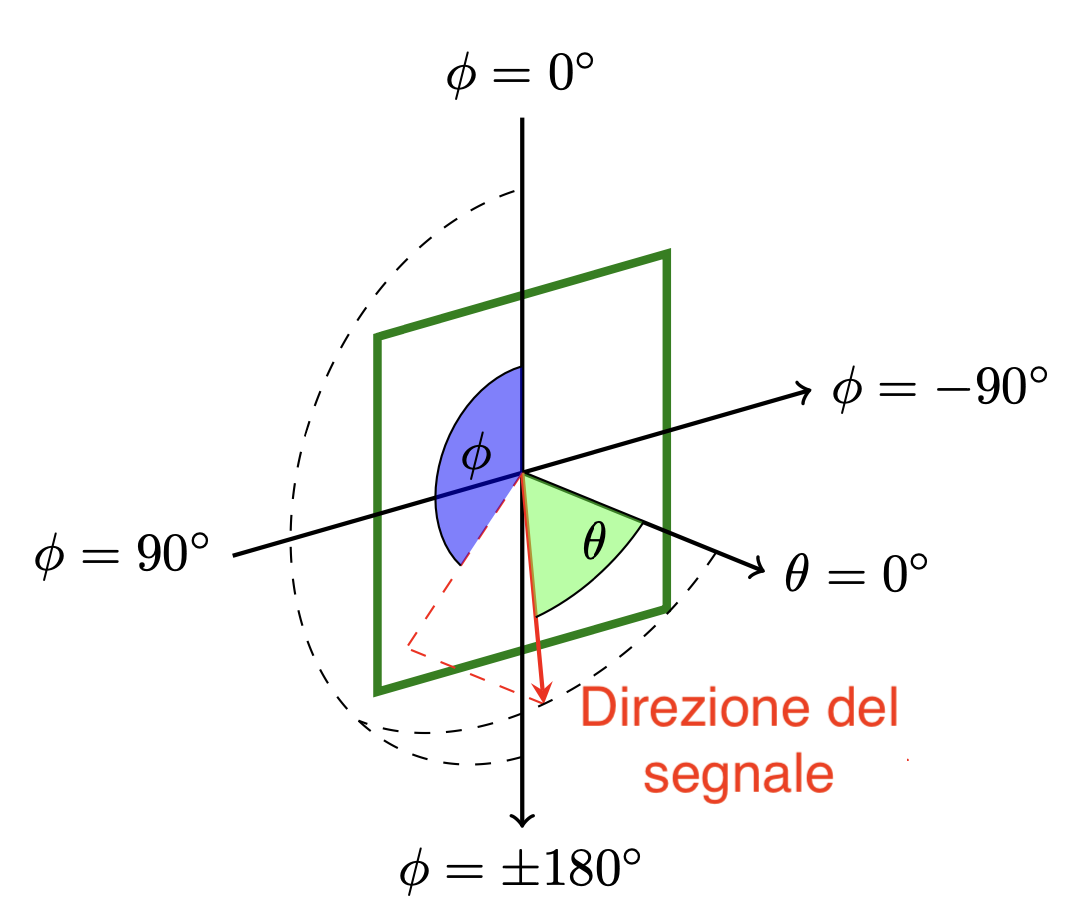
\includegraphics[width=8cm]{images/examples/coords.png}
    \begin{adjustwidth}
      {0pt}{5pt}
      \begin{varwidth}
        {8cm}
        \caption{Angoli di incidenza e riflessione del segnale rispetto la RIS\cite{cooperis}}
        \label{fig:coords}
      \end{varwidth}
    \end{adjustwidth}
  \end{minipage}
  \begin{minipage}[t]{0.5\linewidth}
    \centering
    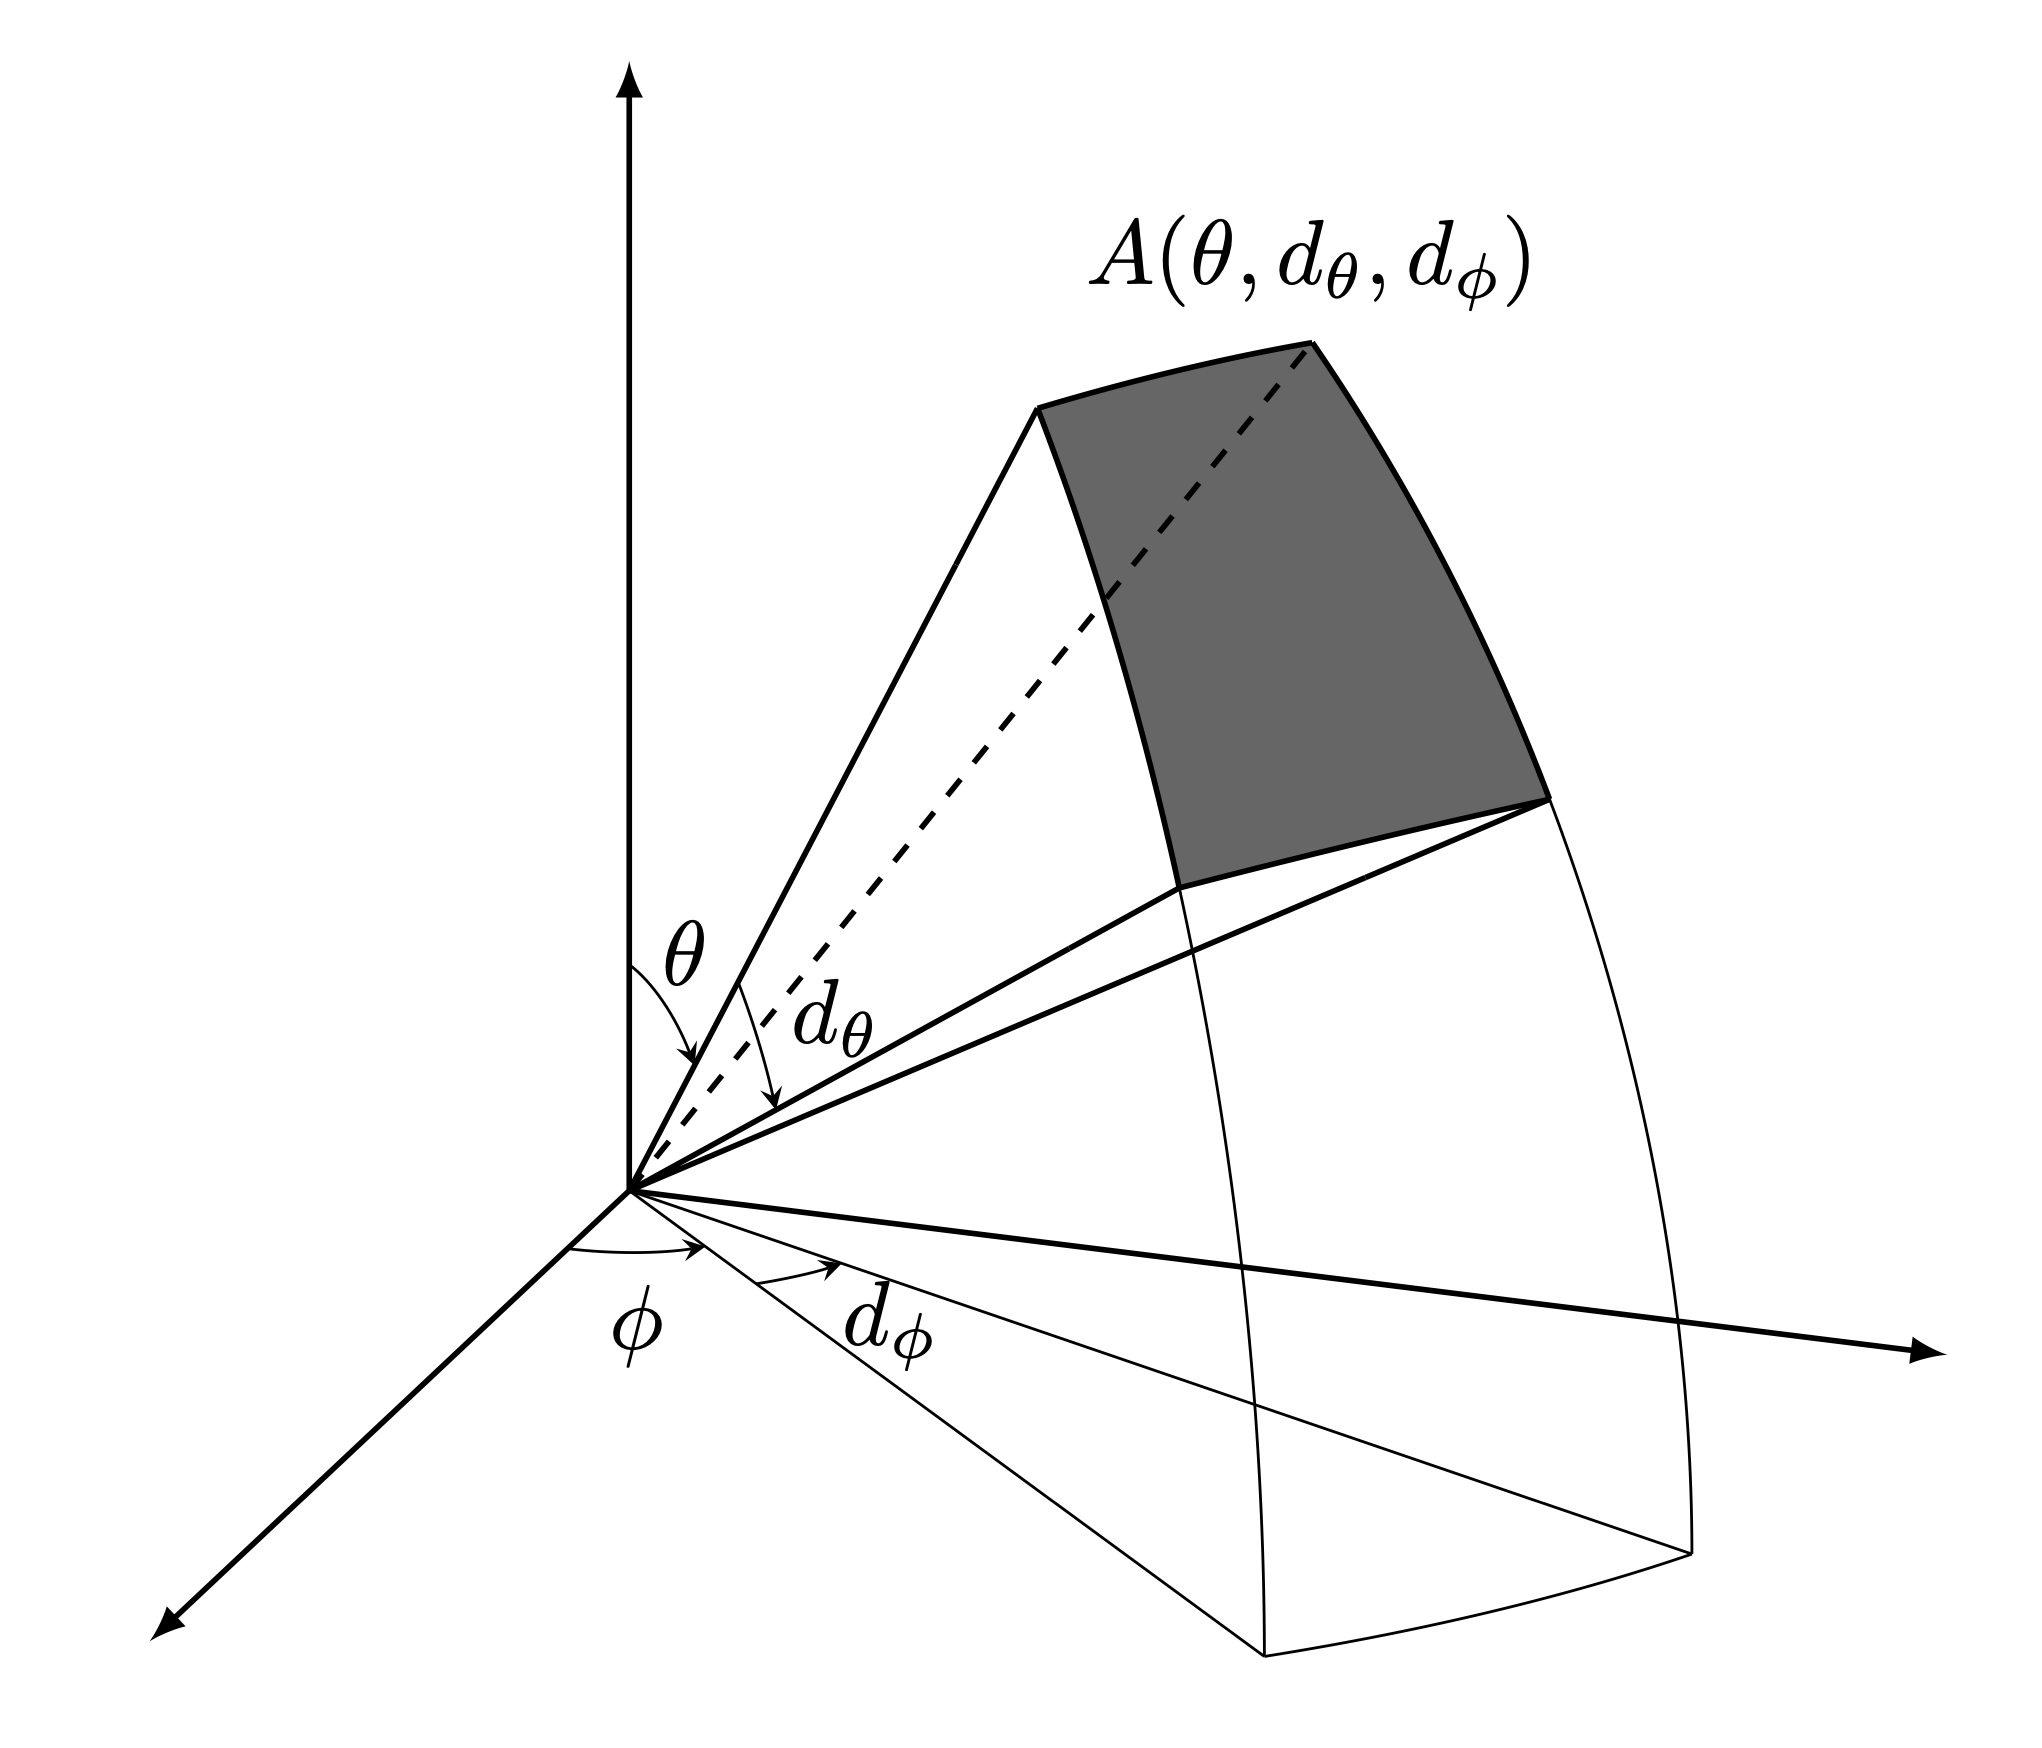
\includegraphics[width=8cm]{images/examples/spherical-element.png}
    \begin{adjustwidth}
      {5pt}{0pt}
      \begin{varwidth}
        {8cm}
        \caption{Esempio grafico di un elemento sferico e la sua
        discretizzazione\cite{cooperis}}
        \label{fig:spherical-elem}
      \end{varwidth}
    \end{adjustwidth}
  \end{minipage}
\end{figure}

L'apprendimento delle Reconfigurable Intelligent Surfaces è fondamentale per comprendere
al meglio quali sono le potenziali criticità e gli eventuali punti di ottimizzazione
della libreria \textit{CoopeRIS}, e di conseguenza di questo elaborato. Come già
accennato nel capitolo \ref{subsec:risframework}, le Reconfigurable Intelligent Surfaces
sono dispositivi che permettono di modificare la riflessione di un segnale appartenente
ad un canale di comunicazione tra un trasmettitore e un ricevitore, al fine di
migliorare la qualità del segnale ricevuto. Questi dispositivi sono composti da un
insieme di elementi radianti, che possono essere attivati per modificare la
riflessione del segnale in arrivo. La somma dei contributi di riflessione di ogni
singolo elemento radiante permette di ottenere un segnale riflesso nitido e direzionato
verso il ricevitore, migliorando così la qualità del segnale ricevuto. La libreria
\textit{CoopeRIS} supporta esclusivamente le RIS passive, ovvero quelle che non permettono
di amplificare il segnale, ma che ne migliorano solo la riflessione. Nel contesto
di una simulazione il parametro più rilevante è $\textbf{G}$, il guadagno
isotropico della RIS dettato dall'equazione \ref{eq:gain}, il quale permette di valutare
la qualità del segnale ricevuto e pertanto la qualità della comunicazione tra trasmettitore
e ricevitore. Esso non è altro che la somma della potenza in \ref{eq:power} del
segnale riflesso in ogni direzione del ricevitore $rx$, normalizzata rispetto all'area
$A(\vartheta, d_{\theta}, d_{\phi})$ del corrispettivo elemento sferico,
definito nell'equazione \ref{eq:area-spherical-element}. Si noti che, per
necessità di calcolo, l'area degli elementi sferici, e di conseguenza anche
$\Theta_{m,n}$ e $\Phi_{m,n}$, deve essere obbligatoriamente resa discreta e la loro
risoluzione angolare è posta pari a $d_{\theta}$ e $d_{\phi}$, rappresentata in
figura \ref{fig:spherical-elem}. In equazione \ref{eq:phase-phi} è definito $\Phi
_{m,n}$ per elemento radiante in posizione $m$, $n$ dato l'angolo di incidenza
$\phi_{i}$ e riflessione $\phi_{r}$. Esso rappresenta lo sfasamento del segnale dovuto
alla attuale configurazione della RIS. In equazione \ref{eq:phase-theta} è
invece denotato lo sfasamento $\Theta_{m,n}$, il quale descrive lo sfasamento dovuto
alla posizione del trasmettitore e ricevitore. Questa differenziazione consente
il calcolo del guadagno della RIS nella condizione in cui l'attuale
configurazione della RIS sia stata determinata con angoli di incidenza e
riflessione dissimili rispetto le attuali posizione del trasmettitore e
ricevitore. Questa combinazione di fattori è il motivo per cui i contributi dei due
sfasamenti sono sommati nel calcolo del guadagno in equazione \ref{eq:power}.
Infine, in tabella \ref{tab:symbols} sono riportati i simboli e le definizioni utilizzate
per la descrizione delle equazioni sopracitate.

\vspace{1em}

\begin{table}[!ht]
  \centering
  \begin{tabular}{p{.15\textwidth}p{.80\textwidth}}
    \hline
    \textbf{Simbolo}                     & \textbf{Significato}                                                                                                                                                                \\
    \hline
    $M$, $N$                             & Grandezza della matrice di elementi radianti                                                                                                                                        \\
    $m$, $n$                             & Indici di posizione degli elementi radianti                                                                                                                                         \\
    $a_{m,n}$                            & Guadagno di ampiezza del singolo elemento ris (in posizione $m$, $n$, in questo modello si assume sempre pari a $1$)                                                                \\
    $\lambda$                            & Lunghezza d'onda del segnale                                                                                                                                                        \\
    $d_{u}$                              & Distanza tra gli elementi radianti                                                                                                                                                  \\
    $\phi$, $\theta$                     & Azimuth ed elevazione del segnale. Diversi pedici indicano rispettivamente il trasmettitore ($tx$), il ricevitore ($rx$), incidenza ($i$) e riflessione ($r$)                       \\
    $\Phi_{m,n}$, $\Theta_{m,n}$         & Sfasamento del singolo elemento radiante (in posizione $m$, $n$) dovuto rispettivamente alla configurazione della RIS e del segnale data la posizione di trasmettitore e ricevitore \\
    $f(\phi, \theta)$                    & Pattern di scattering dell'elemento radiante (in questo modello si assume sempre pari a $1$)                                                                                        \\
    $\textbf{P}_{\phi_{rx},\theta_{rx}}$ & Potenza del segnale riflesso in uscita                                                                                                                                              \\
    $\textbf{G}$                         & Guadagno normalizzato della RIS                                                                                                                                                     \\
    $A(\theta, d_{\theta}, d_{\phi})$    & Area di un elemento sferico per un elevazione $\theta$ e per una risoluzione angolare di elevazione e azimuth $d_{\theta}$ e $d_{\phi}$                                             \\
    \hline
  \end{tabular}
  \caption{Tabella dei simboli}
  \label{tab:symbols}
\end{table}

\begin{equation}
  \label{eq:phase-phi}\Phi_{m,n}= \frac{2\pi d_{u}}{\lambda}[n(\cos{\phi_{r}\sin{\theta_{r}}}
  -\cos{\phi_{i}}\sin{\theta_{i}})+m(\sin{\phi_{r}}\cos{\theta_{r}}-\sin{\phi_{i}}
  \cos{\theta_{i}})]
\end{equation}

\begin{equation}
  \label{eq:phase-theta}\Theta_{m,n}= \frac{2\pi d_{u}}{\lambda}[n(-\cos{\phi_{rx}\sin{\theta_{rx}}}
  +\cos{\phi_{tx}}\sin{\theta_{tx}})+m(-\sin{\phi_{rx}}\cos{\theta_{rx}}+\sin{\phi_{tx}}
  \cos{\theta_{tx}})]
\end{equation}

\begin{equation}
  \label{eq:power}\textbf{P}_{\phi_{rx},\theta_{rx}}= \left|\sum_{m=0}^{M-1}{\sum_{n=0}^{N-1}{f(\phi_{tx}, \theta_{tx})f(\phi_{rx},\theta_{rx})a_{m,n}e^{-j(\Phi_{m,n}+\Theta_{m,n})}}}
  \right|^{2}, \forall \phi_{rx}, \theta_{rx}
\end{equation}

\begin{equation}
  \label{eq:area-spherical-element}A(\theta, d_{\theta}, d_{\phi})=
  \begin{cases}
    d_{\phi}(1-\cos{\frac{d_{\theta}}{2}})                                         & \text{se }\theta = 0                 \\
    d_{\phi}(\cos{\theta-\frac{d_{\theta}}{2}}- \cos{\theta+\frac{d_{\theta}}{2}}) & \text{se }0 < \theta < \frac{\pi}{2} \\
    d_{\phi}(\theta-\frac{d_{\theta}}{2})                                          & \text{se }\theta = \frac{\pi}{2}     \\
  \end{cases}
\end{equation}

\begin{equation}
  \label{eq:gain}\textbf{G}=\textbf{P}\frac{2\pi}{(\textbf{P}^{\top}\cdot
  \mathds{1})^{\top}\cdot A(\vartheta, d_{\theta}, d_{\phi})}
\end{equation}

\section{Parallel Computing}
\label{sec:parallelcomputing}

Con il termine \textit{parallel computing} si intende la divisione di un
problema in sotto-problemi che possono essere risolti in parallelo su più unità
di calcolo. Un unità di calcolo può essere un core di una CPU, un core di una
GPU, un thread di un processore o un processore dedicato. Questa divisione
permette ai calcolatori dotati di più unità di calcolo di risolvere problemi di
dimensioni maggiori in tempi molto più brevi rispetto a calcolatori che non
implementano il parallelismo. La loro comparsa è stato un traguardo storico e fondamentale
per lo sviluppo delle moderne tecnologie informatiche. Questo capitolo si
propone di fornire una panoramica generale sulle tecniche di parallel computing,
con particolare attenzione alle differenze tra CPU e GPU e tra i framework \textit{CUDA}
e \textit{OpenCL}.

\subsection{CPU vs. GPU}
\label{subsec:cpuvsgpu}

Le CPU e le GPU sono due tipologie di unità di calcolo che distinguono per
architettura, scopo e prestazioni. La loro differenziazione nasce dalla natura
delle operazioni che possono essere eseguite su di esse. Generalmente le CPU sono
progettate per eseguire operazioni complesse e molto variegate, forniscono un'architettura
di calcolo più generica e flessibile (\textit{general purpose}) e per questo possono
eseguire parallelamente un numero limitato di operazioni. Le GPU, d'altra parte,
sono specializzate nel parallelizzare le operazioni su grandi quantità di dati, al
costo di una minore flessibilità. Per questa ragione, se prese singolarmente, le
performance delle unità di calcolo sono inferiori rispetto a quelle delle CPU. Per
poter meglio evidenziare le differenze tra le due piattaforme, è necessario
introdurre i concetti di SISD, SIMD e SIMT.

\paragraph{Single Instruction, Single Data (SISD)}
\label{para:simd}

Il modello SISD è quello del calcolo tradizionale ed è il più elementare tra i tre.
Consiste in un'architettura sequenziale in cui un singolo processore esegue un'istruzione
per volta su un singolo dato. Questo modello è tipico delle CPU, che possono
però gestire più thread in parallelo grazie alla presenza di più core
indipendenti che eseguono diverse istruzioni su diversi dati. Questa tecnica è detta
\textit{multi-threading} e permette di eseguire più processi in parallelo. Data la
sua semplicità, il modello SISD permette di ottenere performance elevate su
problemi che richiedono un'elaborazione sequenziale di dati, come ad esempio i sistemi
operativi o i programmi di uso generale.

\begin{figure}[h!]
  \centering
  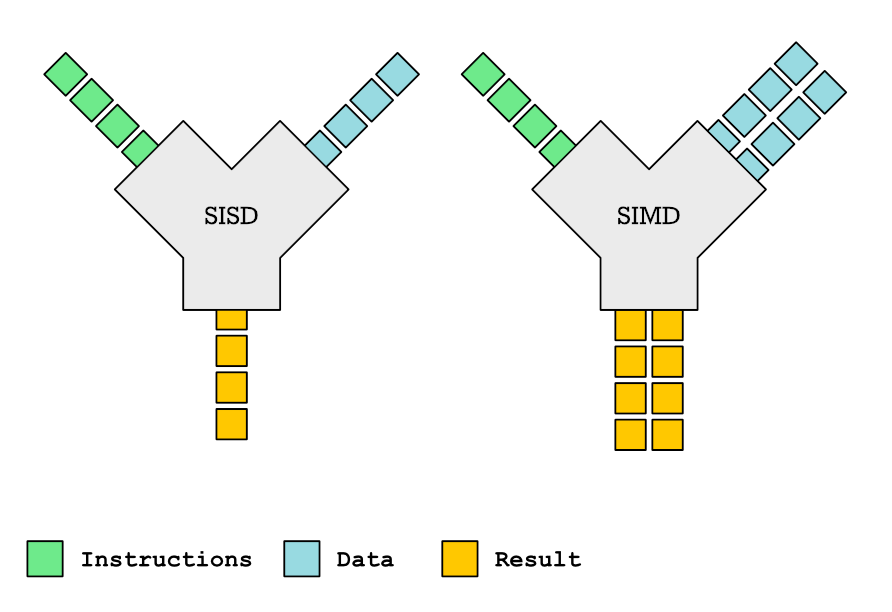
\includegraphics[width=.40\linewidth]{images/examples/sisd-simd.png}
  \caption{Differenza tra SISD e SIMD}
  \label{fig:sisd-simt} \footnotesize{Fonte: \url{https://johnnysswlab.com/crash-course-introduction-to-parallelism-simd-parallelism/}}
\end{figure}

\paragraph{Single Instruction, Multiple Data (SIMD)}
\label{para:simd}

Come suggerisce il nome, la tecnica SIMD permette di eseguire un'istruzione per elaborare
più dati simultaneamente. Questa tecnica è particolarmente efficace per eseguire
operazioni identiche su grandi quantità di dati, come calcoli vettoriali, o
generalmente nelle strutture linearizzabili, come le matrici. La sua
implementazione trova spazio sia nelle GPU che nelle CPU, attraverso l'uso di apposite
istruzioni definite dall'ISA (Instruction Set Architecture) del processore.

\paragraph{Single Instruction, Multiple Threads (SIMT)\cite{generalpurposegpu}}
\label{para:simt}

La tecnica SIMT è una variante della tecnica SIMD che estende il concetto di parallelismo
a livello di thread. Il suo funzionamento consiste in più thread, raggruppati in
gruppi detti \textit{warps}. Ogni thread possiede il proprio insieme di registri
e il proprio contesto, ma condividono l'istruzione da eseguire all'interno del
warp. In questo modo, tutti i thread del \textit{warp} eseguono la medesima istruzione,
ma con dati diversi. Se per l'architettura del nostro programma non tutti i thread
all'interno del \textit{warp} soddisfano un controllo di flusso, ad esempio in un
branch condizionale, allora i thread che non rispettano la condizione vengono
disattivati, mentre quelli che soddisfano la condizione continuano l'esecuzione.
Questo comportamento è detto \textit{divergenza} e può portare a un rallentamento
delle prestazioni del programma, in quanto i thread disattivati devono comunque
attendere il completamento dell'istruzione da parte dei thread attivi, che a loro
volta devono attendere il completamento delle istruzioni presenti nell'altro ramo
del branch condizionale. Le GPU sono i dispositivi che implementano questa
tecnica che è alla base del loro funzionamento.

\vspace{1em}

Queste tecniche sono alla base del funzionamento delle CPU e delle GPU, e
evidenziano quali sono le aree di applicazione di ciascuna di esse. Di seguito,
a titolo esemplificativo, viene riportato un esempio implementativo di due funzioni
di somma di vettori in pseudo-codice, una per CPU (\ref{alg:sumvectorscpu}) e
una per GPU (\ref{alg:sumvectorsgpu}).

\begin{figure}[h!]
  \vspace{1em}
  \begin{algorithm}
    [H]
    \caption{Somma di vettori tramite CPU}
    \label{alg:sumvectorscpu}
    \begin{algorithmic}
      \Function{sum\_vectors\_cpu}{A, B, C} \For{$i \gets 0$ to $n$} \State
      $C[i] \gets A[i] + B[i]$ \EndFor \EndFunction
    \end{algorithmic}
  \end{algorithm}
  \vspace{1em}
\end{figure}

Possiamo notare come la funzione \texttt{sum\_vectors\_cpu} esegua la somma di
due vettori $A$ e $B$ e memorizzi il risultato in un terzo vettore $C$ tramite
un ciclo \texttt{for} che scorre tutti gli elementi dei vettori. Questo
approccio è sequenziale ed è quello classico adotto per l'esecuzione su CPU.

\begin{figure}[h!]
  \vspace{1em}
  \begin{algorithm}
    [H]
    \caption{Somma di vettori tramite GPU}
    \label{alg:sumvectorsgpu}
    \begin{algorithmic}
      \Function{sum\_vectors\_gpu}{A, B, C} \State $i \gets \textit{threadId}$ \State
      $C[i] \gets A[i] + B[i]$ \EndFunction
    \end{algorithmic}
  \end{algorithm}
  \vspace{1em}
\end{figure}

La funzione \textit{sum\_vectors\_gpu}, invece, esegue lo stesso compito tramite
sole due istruzioni, senza necessità di un ciclo \texttt{for}. Questo è possibile
proprio per l'architettura SIMT, poiché $n$ istanze della funzione \texttt{sum\_vectors\_gpu}
vengono eseguite, con $n$ pari al numero di elementi da sommare. Ogni istanza, o
thread, ha associato un indice $i$ che identifica l'elemento del vettore su cui deve
operare, che si ottiene tramite il contesto del thread stesso. In gergo, questa
funzione viene definita \textit{kernel}, ovvero una funzione compilata nel
codice macchina specifico per la GPU, la quale sarà poi invocata dal codice \textit{host},
ovvero il programma che esegue sulla CPU e che gestisce l'esecuzione sul \textit{device}
GPU, tramite le API predisposte dal framework di riferimento.

\subsection[\textit{CUDA} vs. \textit{OpenCL}]{\textit{CUDA} vs. \textit{OpenCL}\cite{cuda}\cite{opencl}\cite{cudavsopencl}}
\label{subsec:cudavsopencl}

\textit{CUDA} e \textit{OpenCL} sono due framework per il parallel computing
piuttosto diffusi e utilizzati per sfruttare le potenzialità delle GPU. Entrambi
i framework permettono di scrivere codice in \textit{C/C++} per creare procedure
eseguibili su GPU, ma differiscono per finalità e prestazioni. \textit{CUDA} è noto
per essere più facile da utilizzare e offre un livello di ottimizzazione superiore.
Tuttavia, questo vantaggio comporta un compromesso significativo: la
compatibilità è limitata esclusivamente alle GPU prodotte da NVIDIA. Questa restrizione
deriva dal fatto che \textit{CUDA} è stato sviluppato e mantenuto interamente da
NVIDIA, rendendolo utilizzabile solo con le loro GPU. \textit{OpenCL}, invece, è
un framework più generico e flessibile, che permette di programmare virtualmente
su tutte le piattaforme GPU, ma al costo di un \textit{overhead} maggiore
rispetto a \textit{CUDA} poiché, ad esempio, è necessario compilare le funzioni \textit{kernel}
a runtime, mentre in \textit{CUDA} questo passaggio è già gestito in fase di
compilazione. Entrambi sono molto diffusi e utilizzati, e la scelta tra uno e l'altro
dipende dalle esigenze del programmatore e dal progetto. Anche se presente, la
loro differenza di prestazioni è trascurabile se si confrontano i risultati in
implementazioni dove le GPU trovano la loro massima efficacia rispetto alle CPU
e se si sanno sfruttare sapientemente le loro potenzialità.

\section{Limiti teorici}
\label{sec:limititeorici}

Sebbene il calcolo parallelo sia una tecnica molto potente, presenta dei limiti
invalicabili che pongono dei vincoli sulle massime prestazioni ottenibili. La comprensione
di questi limiti è fondamentale per la progettazione di sistemi paralleli efficienti,
soprattutto per individuare le parti del codice che sono strategicamente più
importanti da ottimizzare. Il principio di maggiore rilevanza per questo elaborato
è rappresentato dalla Legge di Amdahl, il quale rivestirà un ruolo preponderante
nell'analisi statica condotta sulla libreria in oggetto, come discusso nel paragrafo
\ref{sec:ottimizzazione}. Questo principio sarà fondamentale per identificare le
sezioni del codice che richiedono particolare attenzione e ottimizzazione, consentendo
un miglioramento mirato delle prestazioni complessive del sistema.

\subsection{Legge di Amdahl}
\label{sec:amdahl}

La Legge di Amdahl, formulata da Gene Amdahl nel 1967, è un principio
fondamentale pessimista che descrive un limite superiore al miglioramento
teorico delle prestazioni di un sistema in seguito all'aggiunta di risorse
parallele in funzione della frazione del problema che può beneficiare della
parallelizzazione. La sua formulazione è la seguente:

\begin{equation}
  S(N) = \frac{1}{(1 - P) + \frac{P}{N}}
\end{equation}

Dove:
\begin{itemize}
  \item $S(N)$ è il miglioramento teoretico ottenuto con $N$ processori.

  \item $N$ è il numero di processori.

  \item $P$ è la frazione del problema che può beneficiare della parallelizzazione.
\end{itemize}

In sintesi, questo modello prevede che all'aumentare del numero di processori,
il miglioramento ottenuto con l'aggiunta di un processore aggiuntivo tende a
zero. Per questa ragione, nel paradigma della parallelizzazione, è più conveniente
parallelizzare le parti del codice che richiedono più tempo di esecuzione che aggiungere
processori per parallelizzare parti del codice che richiedono poco tempo di esecuzione.
Inoltre, non sono considerati altri fattori che possono influenzare le prestazioni
di un sistema parallelo, come ad esempio la latenza di comunicazione tra i
processori o il tempo tecnico necessario per l'avvio, la sincronizzazione e la terminazione
dei processi paralleli.
  \chapter{Metodologia e Sviluppo}
\label{ch:metodologiasviluppo}

\section{Descrizione della libreria RIS di base: CoopeRIS}
\label{sec:libreria}

\lipsum[1]

\subsection{Architettura e funzionamento della libreria cooperis}
\label{sec:architettura}

\lipsum[1]

\subsection{Identificazione dei colli di bottiglia e aree di ottimizzazione}
\label{sec:ottimizzazione}

\lipsum[1]

\section{Implementazione della soluzione proposta}
\label{sec:implementazione}

\lipsum[1]

\subsection{Parallelizzazione tramite multi-threading}
\label{subsec:multithreading}

\lipsum[1]

\subsection{Parallelizzazione su GPU}
\label{subsec:cuda}

\lipsum[1]

\section{Discussione e Valutazione}
\label{ch:discussione}

\subsection{Vantaggi delle soluzioni implementate}
\label{subsec:vantaggi}

\lipsum[1]

\paragraph{Performance e tempo di esecuzione}
\label{para:performance}

\lipsum[1]

\paragraph{Supporto multi-piattaforma}
\label{para:supporto}

\lipsum[1]

\subsection{Svantaggi delle soluzioni implementate}
\label{sec:svantaggi}

\lipsum[1]

\paragraph{Leggibilità e manutenibilità del codice}
\label{para:leggibilita}

\lipsum[1]

\paragraph{Richiesta di hardware dedicato}
\label{para:hardware}

\lipsum[1]

\paragraph{Richiesta di conoscenze specifiche}
\label{para:conoscenze}

\lipsum[1]

\subsection{Limiti e sfide affrontate}
\label{subsec:limiti}

\lipsum[1]
  \chapter{Risultati}
\label{ch:risultati}

\section{Metodologia di valutazione}
\label{sec:bencharmking}

\lipsum[1]

\section{Benchmarking della libreria}
\label{sec:benchmarking}

\lipsum[1]

\subsection{Risultati: CPU single-thread vs multi-thread}
\label{subsec:risultati-cpu}

\lipsum[1]

\subsection{Risultati: Cuda vs OpenCL}
\label{subsec:risultati-cuda-opencl}

\lipsum[1]

\subsection{Risultati complessivi}
\label{subsec:risultati-complessivi}

\lipsum[1]

\section{Dimostrazione sul framework}
\label{sec:dimostrazione}

\lipsum[1]

  % Conclusions
  \chapter{Conclusioni}
\label{cha:conclusioni}

La libreria \textit{CoopeRIS} ha dimostrato in modo evidente come il calcolo parallelo
possa essere sfruttato per ottimizzare e accelerare la simulazione di sistemi complessi
come le Reconfigurable Intelligent Surfaces (RIS). Questo elaborato ha permesso
di approfondire le caratteristiche distintive di questa tecnologia innovativa e
di evidenziare le potenzialità dell'approccio parallelo. Nel corso del lavoro,
sono state analizzate le principali differenze tra un approccio di
parallelizzazione basato su CPU e uno su GPU, mettendo in luce vantaggi e svantaggi
di entrambi. Sebbene il processo di sviluppo e ottimizzazione abbia incontrato
alcune limitazioni e criticità, i risultati ottenuti sono stati soddisfacenti e hanno
raggiunto gli obiettivi prefissati. Il progetto ha inoltre consentito di
acquisire nuove competenze e conoscenze, sottolineando le potenzialità del calcolo
parallelo e della programmazione su GPU. Nonostante i progressi compiuti, questo
lavoro rappresenta solo un punto di partenza per ulteriori sviluppi e miglioramenti.
Futuri interventi potrebbero includere l'implementazione di ulteriori micro-ottimizzazioni
o il perfezionamento di altre procedure non ancora ottimizzate. In conclusione,
la libreria \textit{CoopeRIS} si è rivelata un valido caso di studio per l'ottimizzazione
di un sistema complesso e ha perfettamente evidenziato l'efficacia dell'approccio
parallelo nella simulazione di simili sistemi.

  \endgroup

  % Bibliography
  \addcontentsline{toc}{chapter}{Bibliografia}
  % Alphabetical order of authors
  \bibliographystyle{plain}
  \bibliography{bibliography.bib}

  % Attachments
  \titleformat{\chapter} {\normalfont\Huge\bfseries}{Appendice \thechapter}{1em}{}
  \appendix
  \chapter{Codice sorgente rilevante}
\label{cha:codice}

\lipsum[1]

\end{document}